%\documentclass[fleqn, letterpaper]{amsart}
\documentclass[fleqn, letterpaper]{tufte-handout}
\usepackage{times}
\usepackage{amsmath}
\usepackage{amssymb}
\usepackage{graphicx}
\usepackage{booktabs}
\usepackage{multirow}
\usepackage{listings}
\usepackage{epstopdf}
\usepackage{bm}
\usepackage{natbib}
%\usepackage[left=1in]{geometry}

\newcommand{\R}{\mathcal{R}}
\newcommand{\E}{\text{E}}
\newcommand{\p}{p_{XY}}
\newcommand{\T}{^\text{T}}
\renewcommand{\arraystretch}{1.5}

\title{Problem Set 6 --- ENCE689E Spring 2014}
\author{David Prentiss}

\begin{document}
\maketitle

\section{1. Kalman Filter}
See attached.

\section{2. Kalman Filter}

{\scriptsize
        \begin{minipage}{\linewidth}
                \lstinputlisting[language=Matlab, caption={Propagation of a linear soil moisture model},
                basicstyle=\ttfamily, label=lst1]{ps6.m}
        \end{minipage}
}

\subsection{(a)}
\begin{align*}
\begin{pmatrix}
\mathbf{y}_{t+1} \\
\mathbf{u}_{t+1} \\
\end{pmatrix}
&=
\begin{pmatrix}
a\mathbf{y}_t + \mathbf{u}_t \\
\rho\mathbf{u}^{(true)}_t+ \mathbf{w}_t
\end{pmatrix}
\end{align*}

\subsection{(b)}

\subsection{(c)}
See figures \ref{2ca} and \ref{2cb}.
\begin{figure}
        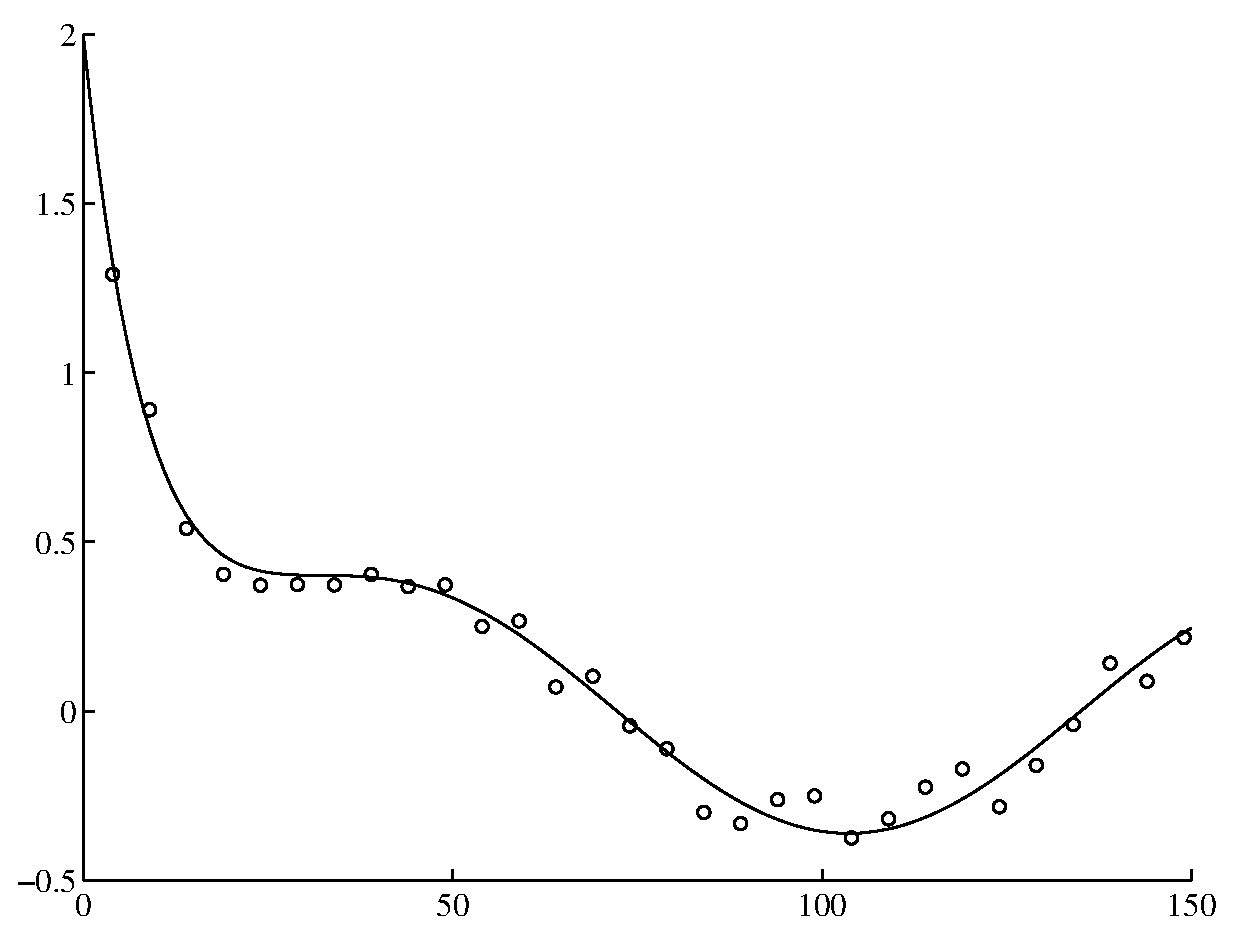
\includegraphics[width=\textwidth]{2ca}
        \caption{True, single-state system and simulated measurement error.}
        \label{2ca}
\end{figure}
\begin{figure}
        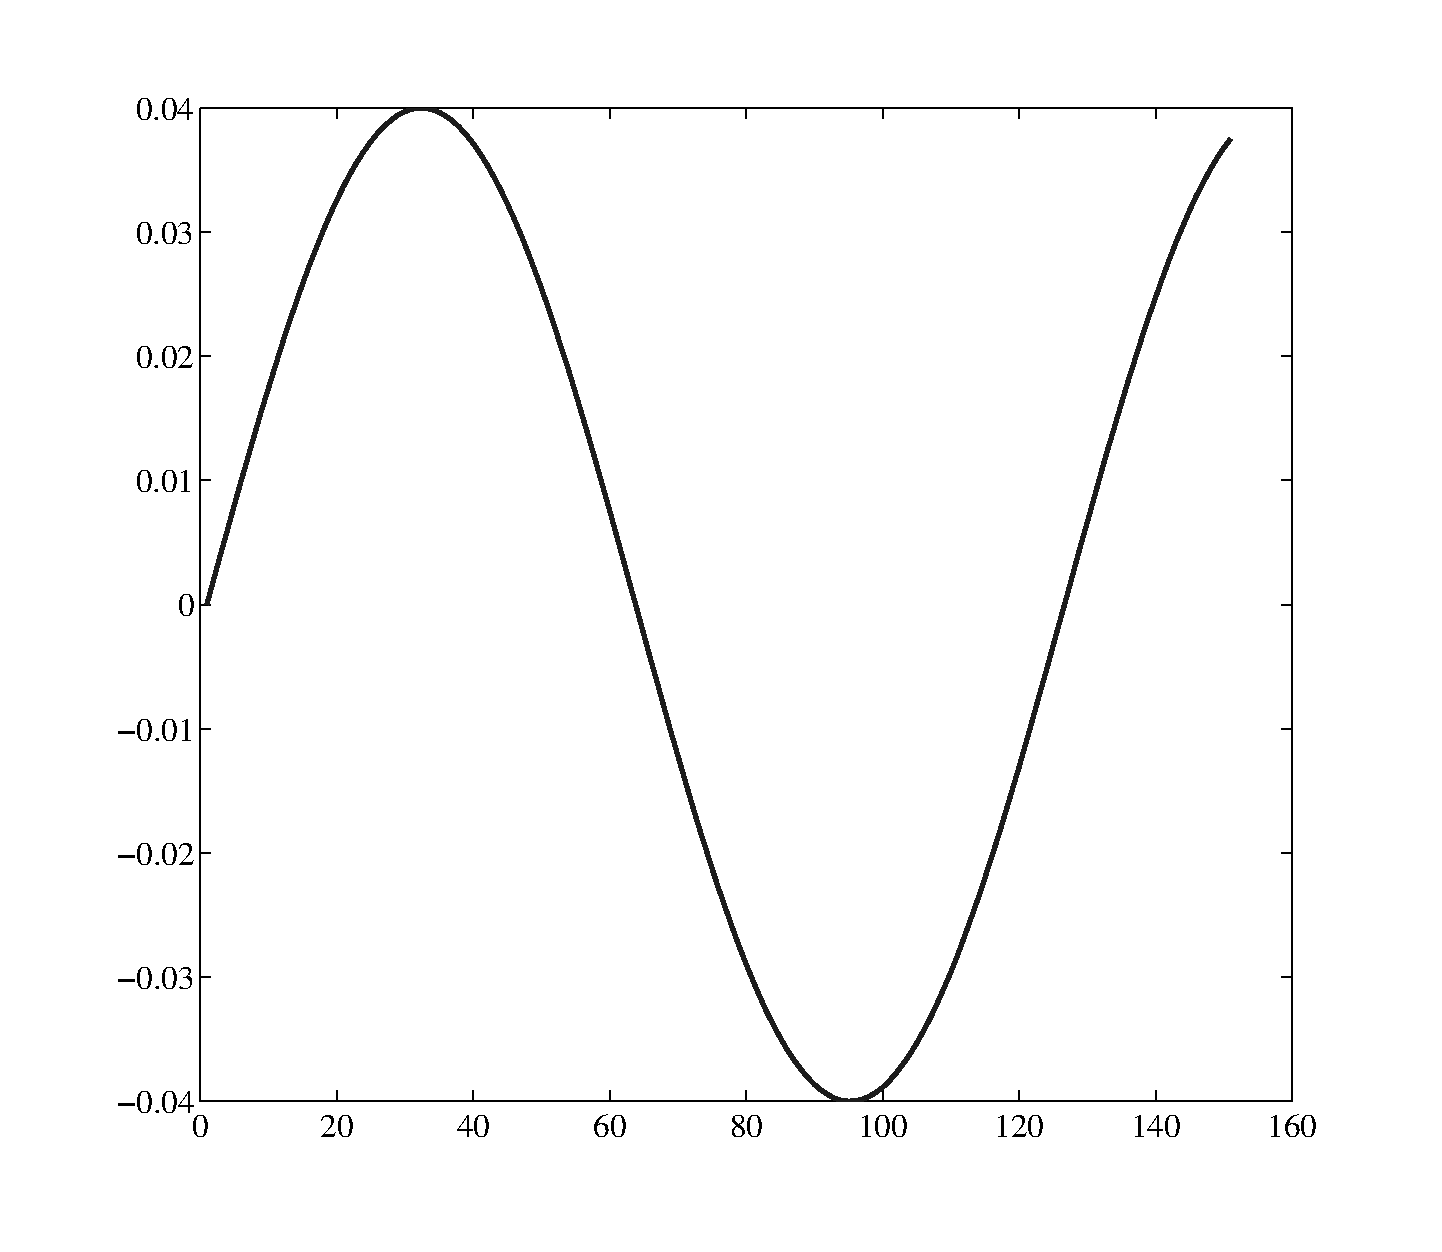
\includegraphics[width=\textwidth]{2cb}
        \caption{True model forcing}
        \label{2cb}
\end{figure}

\subsection{(d)}
\subsection{(e)}
\subsection{(f)}
\subsection{(g)}

\end{document}